\documentclass[twoside]{book}

% Packages required by doxygen
\usepackage{fixltx2e}
\usepackage{calc}
\usepackage{doxygen}
\usepackage[export]{adjustbox} % also loads graphicx
\usepackage{graphicx}
\usepackage[utf8]{inputenc}
\usepackage{makeidx}
\usepackage{multicol}
\usepackage{multirow}
\PassOptionsToPackage{warn}{textcomp}
\usepackage{textcomp}
\usepackage[nointegrals]{wasysym}
\usepackage[table]{xcolor}

% Font selection
\usepackage[T1]{fontenc}
\usepackage[scaled=.90]{helvet}
\usepackage{courier}
\usepackage{amssymb}
\usepackage{sectsty}
\renewcommand{\familydefault}{\sfdefault}
\allsectionsfont{%
  \fontseries{bc}\selectfont%
  \color{darkgray}%
}
\renewcommand{\DoxyLabelFont}{%
  \fontseries{bc}\selectfont%
  \color{darkgray}%
}
\newcommand{\+}{\discretionary{\mbox{\scriptsize$\hookleftarrow$}}{}{}}

% Page & text layout
\usepackage{geometry}
\geometry{%
  a4paper,%
  top=2.5cm,%
  bottom=2.5cm,%
  left=2.5cm,%
  right=2.5cm%
}
\tolerance=750
\hfuzz=15pt
\hbadness=750
\setlength{\emergencystretch}{15pt}
\setlength{\parindent}{0cm}
\setlength{\parskip}{3ex plus 2ex minus 2ex}
\makeatletter
\renewcommand{\paragraph}{%
  \@startsection{paragraph}{4}{0ex}{-1.0ex}{1.0ex}{%
    \normalfont\normalsize\bfseries\SS@parafont%
  }%
}
\renewcommand{\subparagraph}{%
  \@startsection{subparagraph}{5}{0ex}{-1.0ex}{1.0ex}{%
    \normalfont\normalsize\bfseries\SS@subparafont%
  }%
}
\makeatother

% Headers & footers
\usepackage{fancyhdr}
\pagestyle{fancyplain}
\fancyhead[LE]{\fancyplain{}{\bfseries\thepage}}
\fancyhead[CE]{\fancyplain{}{}}
\fancyhead[RE]{\fancyplain{}{\bfseries\leftmark}}
\fancyhead[LO]{\fancyplain{}{\bfseries\rightmark}}
\fancyhead[CO]{\fancyplain{}{}}
\fancyhead[RO]{\fancyplain{}{\bfseries\thepage}}
\fancyfoot[LE]{\fancyplain{}{}}
\fancyfoot[CE]{\fancyplain{}{}}
\fancyfoot[RE]{\fancyplain{}{\bfseries\scriptsize Generated by Doxygen }}
\fancyfoot[LO]{\fancyplain{}{\bfseries\scriptsize Generated by Doxygen }}
\fancyfoot[CO]{\fancyplain{}{}}
\fancyfoot[RO]{\fancyplain{}{}}
\renewcommand{\footrulewidth}{0.4pt}
\renewcommand{\chaptermark}[1]{%
  \markboth{#1}{}%
}
\renewcommand{\sectionmark}[1]{%
  \markright{\thesection\ #1}%
}

% Indices & bibliography
\usepackage{natbib}
\usepackage[titles]{tocloft}
\setcounter{tocdepth}{3}
\setcounter{secnumdepth}{5}
\makeindex

% Hyperlinks (required, but should be loaded last)
\usepackage{ifpdf}
\ifpdf
  \usepackage[pdftex,pagebackref=true]{hyperref}
\else
  \usepackage[ps2pdf,pagebackref=true]{hyperref}
\fi
\hypersetup{%
  colorlinks=true,%
  linkcolor=blue,%
  citecolor=blue,%
  unicode%
}

% Custom commands
\newcommand{\clearemptydoublepage}{%
  \newpage{\pagestyle{empty}\cleardoublepage}%
}

\usepackage{caption}
\captionsetup{labelsep=space,justification=centering,font={bf},singlelinecheck=off,skip=4pt,position=top}

%===== C O N T E N T S =====

\begin{document}

% Titlepage & ToC
\hypersetup{pageanchor=false,
             bookmarksnumbered=true,
             pdfencoding=unicode
            }
\pagenumbering{alph}
\begin{titlepage}
\vspace*{7cm}
\begin{center}%
{\Large M\+T\+Unit\+Helper Help \\[1ex]\large v1.\+0 }\\
\vspace*{1cm}
{\large Generated by Doxygen 1.8.14}\\
\end{center}
\end{titlepage}
\clearemptydoublepage
\pagenumbering{roman}
\tableofcontents
\clearemptydoublepage
\pagenumbering{arabic}
\hypersetup{pageanchor=true}

%--- Begin generated contents ---
\chapter{R\+E\+A\+D\+ME}
\label{index}\hypertarget{index}{}\section*{M\+T\+Unit\+Helper -\/ A Toolchain to Automate M\+T\+Unit}

The problem of Unit Testing in Meta\+Trader is that there is a lack of pre-\/developed testing frameworks, such as Google Test, j\+Unit, Cpp\+Test and so on.

This project is part of a bigger project called\+: M\+T\+Unit -\/ A Unit Test framework for Meta\+Trader 5. M\+T\+Unit Project can be found here\+: \href{https://github.com/rodrigoshaller/MTUnit}{\tt https\+://github.\+com/rodrigoshaller/\+M\+T\+Unit} and it consists basically in a home made Unit Test Framework developed for Meta\+Trader 5 (yes, you can use it in Meta\+Trader 4, maybe some adjusts need to be made, but it won\textquotesingle{}t be a big deal, I promise).

Let\textquotesingle{}s make something clear\+: \subsubsection*{This project is not a Unit Test! M\+T\+Unit is!}

\subsubsection*{This project is a toolchain intended to make our lives easier in terms of writing Test Suites and Test Cases.}

I\textquotesingle{}ll briefly explain each tool, but for a more complete explanation, I suggest you to read my M\+T\+Unit Project.

\subsubsection*{Tool\+: \mbox{\hyperlink{class_m_t_unit_tests_compiler}{M\+T\+Unit\+Tests\+Compiler}}}

This is the most important tool here. It scans the Test directory and goes through all test files looking for every Test Suite and their respective Test Cases.

Then , it writes a file called \mbox{\hyperlink{_m_t_unit_all_tests_8mqh}{M\+T\+Unit\+All\+Tests.\+mqh}} containing all basic declarations you would have had to write manually.

You can use it by two different ways\+: Directly, or as a Watcher.

What do I mean by \char`\"{}directly\char`\"{}? You can call the mt\+Unit\+Helper.\+exe file passing the argument\+: mt\+Unit\+Tests\+Compiler, and it will generate the \mbox{\hyperlink{_m_t_unit_all_tests_8mqh}{M\+T\+Unit\+All\+Tests.\+mqh}} file once.

Or you can use it as a Watcher. In this case, if you run the mt\+Unit\+Helper.\+exe without any argument (simple double click on the .exe file), the app will enter in a Watcher mode.

In this mode, it will monitors the Test folder and trigger whenever a change is made to that directory. \begin{DoxyWarning}{Warning}
In this case, the app will keep running until you close it.
\end{DoxyWarning}
\subsubsection*{Tool\+: \mbox{\hyperlink{class_m_t_unit_e_a_linker}{M\+T\+Unit\+E\+A\+Linker}}}

This tool is used to update the config files required by the Meta\+Terminal when running an Expert Advisor.

It looks for the EA Parameter and updates it with the name of the generated .ex5 file. \begin{DoxyNote}{Note}
In order to use this tool, the argument received by mt\+Unit\+Helper.\+exe must be\+: mt\+Unit\+E\+A\+Linker Write\+Here\+The\+Path\+Of\+The\+E\+A\+You\+Want\+To\+Run.\+mq5
\end{DoxyNote}
\subsubsection*{Tool\+: \mbox{\hyperlink{class_m_t_unit_logger}{M\+T\+Unit\+Logger}}}

This tool looks for the output log file generated by Meta\+Editor, hijacks this file to the Runners folder and adds some color to the output to make it more visual effective. \begin{DoxyNote}{Note}
In order to use this class, the argument received by mt\+Unit\+Helper.\+exe must be\+: mt\+Unit\+Logger 
\end{DoxyNote}
\begin{DoxyWarning}{Warning}
The colored output does not work directly from Meta\+Editor, so if you want to use it, I suggest you to follow the instructions (M\+T\+Unit Project) for using this tool in Sublime Text 3.
\end{DoxyWarning}
If you didn\textquotesingle{}t take a look at the M\+T\+Unit Project, you may be wondering why \mbox{\hyperlink{class_m_t_unit_e_a_linker}{M\+T\+Unit\+E\+A\+Linker}} and \mbox{\hyperlink{class_m_t_unit_logger}{M\+T\+Unit\+Logger}} are used for. Doesn\textquotesingle{}t Meta\+Editor links to my EA and output the log\+File?

Yes it does. But, as referenced in the M\+T\+Unit Project, I don\textquotesingle{}t like to use the Meta\+Editor. So I\textquotesingle{}ve configured Sublime Text 3 to build and run everything automatically with the press of a button (F7). And that\textquotesingle{}s where the need to develop this 2 tools came from.

So, if you are not planning to use Sublime Text or any other tool for developing Expert Advisors, \mbox{\hyperlink{class_m_t_unit_e_a_linker}{M\+T\+Unit\+E\+A\+Linker}} and \mbox{\hyperlink{class_m_t_unit_logger}{M\+T\+Unit\+Logger}} won\textquotesingle{}t be useful for you.

I suggest you to simply double click on mt\+Unit\+Helper.\+exe before start coding your E\+As and it will manage your tests automatically for you.

\subsubsection*{Other Thoughts}

If you are asking yourself why isn\textquotesingle{}t this project inside M\+T\+Unit Project... I decided to make this a separate project because\+:
\begin{DoxyItemize}
\item It is a separate project. M\+T\+Unit is a Unit Test Framework... M\+T\+Unit\+Helper is not.
\item This project can be adapted for your own needs. It doesn\textquotesingle{}t need to be exclusive for M\+T5. (It is written in C++ using Q\+T\+Creator, btw)
\end{DoxyItemize}

\begin{DoxyNote}{Note}
In order to work, the file structure must follow the structure of this project. An by saying that I mean that the mt\+Unit\+Helper.\+exe file must be inside the \char`\"{}\+Runners\char`\"{} folder and the tests must be placed inside a \char`\"{}\+Test\char`\"{} folder. The \mbox{\hyperlink{_m_t_unit_all_tests_8mqh}{M\+T\+Unit\+All\+Tests.\+mqh}} will be generated inside a \char`\"{}\+Include\char`\"{} folder.
\end{DoxyNote}
That\textquotesingle{}s it. Just let me know if you have any suggestions, critiques or doubts.

Cheers,

Rodrigo Haller (\href{mailto:rodrigoshaller@gmail.com}{\tt rodrigoshaller@gmail.\+com})

This project is made under G\+NU General Public License 
\chapter{Hierarchical Index}
\section{Class Hierarchy}
This inheritance list is sorted roughly, but not completely, alphabetically\+:\begin{DoxyCompactList}
\item \contentsline{section}{M\+T\+Unit\+All\+Tests}{\pageref{class_m_t_unit_all_tests}}{}
\item \contentsline{section}{M\+T\+Unit\+E\+A\+Linker}{\pageref{class_m_t_unit_e_a_linker}}{}
\item \contentsline{section}{M\+T\+Unit\+Logger}{\pageref{class_m_t_unit_logger}}{}
\item \contentsline{section}{My\+Basic\+Test\+Suite}{\pageref{class_my_basic_test_suite}}{}
\item \contentsline{section}{My\+Class\+Testing\+Test\+Suite}{\pageref{class_my_class_testing_test_suite}}{}
\item \contentsline{section}{My\+Global\+Scope\+Test\+Suite}{\pageref{class_my_global_scope_test_suite}}{}
\item Q\+Object\begin{DoxyCompactList}
\item \contentsline{section}{M\+T\+Unit\+Tests\+Compiler}{\pageref{class_m_t_unit_tests_compiler}}{}
\end{DoxyCompactList}
\item Sample\+Class\+To\+Test\begin{DoxyCompactList}
\item \contentsline{section}{My\+Inherited\+Test\+Suite}{\pageref{class_my_inherited_test_suite}}{}
\end{DoxyCompactList}
\end{DoxyCompactList}

\chapter{Class Index}
\section{Class List}
Here are the classes, structs, unions and interfaces with brief descriptions\+:\begin{DoxyCompactList}
\item\contentsline{section}{\mbox{\hyperlink{class_m_t_unit_all_tests}{M\+T\+Unit\+All\+Tests}} }{\pageref{class_m_t_unit_all_tests}}{}
\item\contentsline{section}{\mbox{\hyperlink{class_m_t_unit_e_a_linker}{M\+T\+Unit\+E\+A\+Linker}} }{\pageref{class_m_t_unit_e_a_linker}}{}
\item\contentsline{section}{\mbox{\hyperlink{class_m_t_unit_logger}{M\+T\+Unit\+Logger}} }{\pageref{class_m_t_unit_logger}}{}
\item\contentsline{section}{\mbox{\hyperlink{class_m_t_unit_tests_compiler}{M\+T\+Unit\+Tests\+Compiler}} }{\pageref{class_m_t_unit_tests_compiler}}{}
\item\contentsline{section}{\mbox{\hyperlink{class_my_basic_test_suite}{My\+Basic\+Test\+Suite}} \\*Example of Test Suite }{\pageref{class_my_basic_test_suite}}{}
\item\contentsline{section}{\mbox{\hyperlink{class_my_class_testing_test_suite}{My\+Class\+Testing\+Test\+Suite}} \\*Example of Test Suite }{\pageref{class_my_class_testing_test_suite}}{}
\item\contentsline{section}{\mbox{\hyperlink{class_my_global_scope_test_suite}{My\+Global\+Scope\+Test\+Suite}} \\*Example of Test Suite }{\pageref{class_my_global_scope_test_suite}}{}
\item\contentsline{section}{\mbox{\hyperlink{class_my_inherited_test_suite}{My\+Inherited\+Test\+Suite}} \\*Example of Test Suite }{\pageref{class_my_inherited_test_suite}}{}
\end{DoxyCompactList}

\chapter{File Index}
\section{File List}
Here is a list of all files with brief descriptions\+:\begin{DoxyCompactList}
\item\contentsline{section}{Include/\mbox{\hyperlink{_m_t_unit_all_tests_8mqh}{M\+T\+Unit\+All\+Tests.\+mqh}} \\*This file is auto generated. It contains all tests that the unit test will run }{\pageref{_m_t_unit_all_tests_8mqh}}{}
\item\contentsline{section}{Source/\mbox{\hyperlink{main_8cpp}{main.\+cpp}} \\*This app was made to automate Unit Testing in M\+Q\+L5 }{\pageref{main_8cpp}}{}
\item\contentsline{section}{Source/\mbox{\hyperlink{mt_unit_e_a_linker_8cpp}{mt\+Unit\+E\+A\+Linker.\+cpp}} \\*Update the config filed required by the Meta\+Terminal when running an Expert Advisor }{\pageref{mt_unit_e_a_linker_8cpp}}{}
\item\contentsline{section}{Source/\mbox{\hyperlink{mt_unit_e_a_linker_8h}{mt\+Unit\+E\+A\+Linker.\+h}} \\*Update the config filed required by the Meta\+Terminal when running an Expert Advisor }{\pageref{mt_unit_e_a_linker_8h}}{}
\item\contentsline{section}{Source/\mbox{\hyperlink{mt_unit_logger_8cpp}{mt\+Unit\+Logger.\+cpp}} \\*Hijacks the Log\+File and add colors to the output }{\pageref{mt_unit_logger_8cpp}}{}
\item\contentsline{section}{Source/\mbox{\hyperlink{mt_unitlogger_8h}{mt\+Unitlogger.\+h}} \\*Hijacks the Log\+File and add colors to the output }{\pageref{mt_unitlogger_8h}}{}
\item\contentsline{section}{Source/\mbox{\hyperlink{mt_unit_tests_compiler_8cpp}{mt\+Unit\+Tests\+Compiler.\+cpp}} \\*Scan all Test Files and generates the \mbox{\hyperlink{_m_t_unit_all_tests_8mqh}{M\+T\+Unit\+All\+Tests.\+mqh}} file }{\pageref{mt_unit_tests_compiler_8cpp}}{}
\item\contentsline{section}{Source/\mbox{\hyperlink{mt_unit_tests_compiler_8h}{mt\+Unit\+Tests\+Compiler.\+h}} \\*Scan all Test Files and generates the \mbox{\hyperlink{_m_t_unit_all_tests_8mqh}{M\+T\+Unit\+All\+Tests.\+mqh}} file }{\pageref{mt_unit_tests_compiler_8h}}{}
\item\contentsline{section}{Test/\mbox{\hyperlink{_basic_test_suite___test_8mqh}{Basic\+Test\+Suite\+\_\+\+Test.\+mqh}} \\*File containing the implementation of all Unit Test methods }{\pageref{_basic_test_suite___test_8mqh}}{}
\end{DoxyCompactList}

\chapter{Class Documentation}
\hypertarget{class_m_t_unit_all_tests}{}\section{M\+T\+Unit\+All\+Tests Class Reference}
\label{class_m_t_unit_all_tests}\index{M\+T\+Unit\+All\+Tests@{M\+T\+Unit\+All\+Tests}}
\subsection*{Public Member Functions}
\begin{DoxyCompactItemize}
\item 
\mbox{\hyperlink{class_m_t_unit_all_tests_a77411abf2fe3fcee948cb82357acb722}{M\+T\+Unit\+All\+Tests}} ()
\item 
\mbox{\hyperlink{class_m_t_unit_all_tests_a2d9dccb31b2ce7cd3dc164c0c9c79c8c}{$\sim$\+M\+T\+Unit\+All\+Tests}} ()
\item 
void \mbox{\hyperlink{class_m_t_unit_all_tests_acb555e1d5ff6afa8a5fdbf097abe70f5}{run\+All\+Tests}} ()
\end{DoxyCompactItemize}


\subsection{Detailed Description}


Definition at line 20 of file M\+T\+Unit\+All\+Tests.\+mqh.



\subsection{Constructor \& Destructor Documentation}
\mbox{\Hypertarget{class_m_t_unit_all_tests_a77411abf2fe3fcee948cb82357acb722}\label{class_m_t_unit_all_tests_a77411abf2fe3fcee948cb82357acb722}} 
\index{M\+T\+Unit\+All\+Tests@{M\+T\+Unit\+All\+Tests}!M\+T\+Unit\+All\+Tests@{M\+T\+Unit\+All\+Tests}}
\index{M\+T\+Unit\+All\+Tests@{M\+T\+Unit\+All\+Tests}!M\+T\+Unit\+All\+Tests@{M\+T\+Unit\+All\+Tests}}
\subsubsection{\texorpdfstring{M\+T\+Unit\+All\+Tests()}{MTUnitAllTests()}}
{\footnotesize\ttfamily M\+T\+Unit\+All\+Tests\+::\+M\+T\+Unit\+All\+Tests (\begin{DoxyParamCaption}{ }\end{DoxyParamCaption})\hspace{0.3cm}{\ttfamily [inline]}}



Definition at line 23 of file M\+T\+Unit\+All\+Tests.\+mqh.

\mbox{\Hypertarget{class_m_t_unit_all_tests_a2d9dccb31b2ce7cd3dc164c0c9c79c8c}\label{class_m_t_unit_all_tests_a2d9dccb31b2ce7cd3dc164c0c9c79c8c}} 
\index{M\+T\+Unit\+All\+Tests@{M\+T\+Unit\+All\+Tests}!````~M\+T\+Unit\+All\+Tests@{$\sim$\+M\+T\+Unit\+All\+Tests}}
\index{````~M\+T\+Unit\+All\+Tests@{$\sim$\+M\+T\+Unit\+All\+Tests}!M\+T\+Unit\+All\+Tests@{M\+T\+Unit\+All\+Tests}}
\subsubsection{\texorpdfstring{$\sim$\+M\+T\+Unit\+All\+Tests()}{~MTUnitAllTests()}}
{\footnotesize\ttfamily M\+T\+Unit\+All\+Tests\+::$\sim$\+M\+T\+Unit\+All\+Tests (\begin{DoxyParamCaption}{ }\end{DoxyParamCaption})\hspace{0.3cm}{\ttfamily [inline]}}



Definition at line 24 of file M\+T\+Unit\+All\+Tests.\+mqh.



\subsection{Member Function Documentation}
\mbox{\Hypertarget{class_m_t_unit_all_tests_acb555e1d5ff6afa8a5fdbf097abe70f5}\label{class_m_t_unit_all_tests_acb555e1d5ff6afa8a5fdbf097abe70f5}} 
\index{M\+T\+Unit\+All\+Tests@{M\+T\+Unit\+All\+Tests}!run\+All\+Tests@{run\+All\+Tests}}
\index{run\+All\+Tests@{run\+All\+Tests}!M\+T\+Unit\+All\+Tests@{M\+T\+Unit\+All\+Tests}}
\subsubsection{\texorpdfstring{run\+All\+Tests()}{runAllTests()}}
{\footnotesize\ttfamily void M\+T\+Unit\+All\+Tests\+::run\+All\+Tests (\begin{DoxyParamCaption}{ }\end{DoxyParamCaption})\hspace{0.3cm}{\ttfamily [inline]}}



Definition at line 25 of file M\+T\+Unit\+All\+Tests.\+mqh.



The documentation for this class was generated from the following file\+:\begin{DoxyCompactItemize}
\item 
Include/\mbox{\hyperlink{_m_t_unit_all_tests_8mqh}{M\+T\+Unit\+All\+Tests.\+mqh}}\end{DoxyCompactItemize}

\hypertarget{class_m_t_unit_e_a_linker}{}\section{M\+T\+Unit\+E\+A\+Linker Class Reference}
\label{class_m_t_unit_e_a_linker}\index{M\+T\+Unit\+E\+A\+Linker@{M\+T\+Unit\+E\+A\+Linker}}


{\ttfamily \#include $<$mt\+Unit\+E\+A\+Linker.\+h$>$}

\subsection*{Public Member Functions}
\begin{DoxyCompactItemize}
\item 
\mbox{\hyperlink{class_m_t_unit_e_a_linker_aed54a414af8bd724598a620e60e0ed08}{M\+T\+Unit\+E\+A\+Linker}} ()
\item 
\mbox{\hyperlink{class_m_t_unit_e_a_linker_ac9e5096b4e07298672b442e28ea96880}{$\sim$\+M\+T\+Unit\+E\+A\+Linker}} ()
\item 
int \mbox{\hyperlink{class_m_t_unit_e_a_linker_acf164d0bb5d6769c83832fdcfb45d763}{start}} (Q\+String root\+Dir, Q\+String ea\+Path)
\begin{DoxyCompactList}\small\item\em Open the config file and edit the EA parameter. \end{DoxyCompactList}\end{DoxyCompactItemize}


\subsection{Detailed Description}


Definition at line 22 of file mt\+Unit\+E\+A\+Linker.\+h.



\subsection{Constructor \& Destructor Documentation}
\mbox{\Hypertarget{class_m_t_unit_e_a_linker_aed54a414af8bd724598a620e60e0ed08}\label{class_m_t_unit_e_a_linker_aed54a414af8bd724598a620e60e0ed08}} 
\index{M\+T\+Unit\+E\+A\+Linker@{M\+T\+Unit\+E\+A\+Linker}!M\+T\+Unit\+E\+A\+Linker@{M\+T\+Unit\+E\+A\+Linker}}
\index{M\+T\+Unit\+E\+A\+Linker@{M\+T\+Unit\+E\+A\+Linker}!M\+T\+Unit\+E\+A\+Linker@{M\+T\+Unit\+E\+A\+Linker}}
\subsubsection{\texorpdfstring{M\+T\+Unit\+E\+A\+Linker()}{MTUnitEALinker()}}
{\footnotesize\ttfamily M\+T\+Unit\+E\+A\+Linker\+::\+M\+T\+Unit\+E\+A\+Linker (\begin{DoxyParamCaption}{ }\end{DoxyParamCaption})\hspace{0.3cm}{\ttfamily [inline]}}



Definition at line 25 of file mt\+Unit\+E\+A\+Linker.\+h.

\mbox{\Hypertarget{class_m_t_unit_e_a_linker_ac9e5096b4e07298672b442e28ea96880}\label{class_m_t_unit_e_a_linker_ac9e5096b4e07298672b442e28ea96880}} 
\index{M\+T\+Unit\+E\+A\+Linker@{M\+T\+Unit\+E\+A\+Linker}!````~M\+T\+Unit\+E\+A\+Linker@{$\sim$\+M\+T\+Unit\+E\+A\+Linker}}
\index{````~M\+T\+Unit\+E\+A\+Linker@{$\sim$\+M\+T\+Unit\+E\+A\+Linker}!M\+T\+Unit\+E\+A\+Linker@{M\+T\+Unit\+E\+A\+Linker}}
\subsubsection{\texorpdfstring{$\sim$\+M\+T\+Unit\+E\+A\+Linker()}{~MTUnitEALinker()}}
{\footnotesize\ttfamily M\+T\+Unit\+E\+A\+Linker\+::$\sim$\+M\+T\+Unit\+E\+A\+Linker (\begin{DoxyParamCaption}{ }\end{DoxyParamCaption})\hspace{0.3cm}{\ttfamily [inline]}}



Definition at line 26 of file mt\+Unit\+E\+A\+Linker.\+h.



\subsection{Member Function Documentation}
\mbox{\Hypertarget{class_m_t_unit_e_a_linker_acf164d0bb5d6769c83832fdcfb45d763}\label{class_m_t_unit_e_a_linker_acf164d0bb5d6769c83832fdcfb45d763}} 
\index{M\+T\+Unit\+E\+A\+Linker@{M\+T\+Unit\+E\+A\+Linker}!start@{start}}
\index{start@{start}!M\+T\+Unit\+E\+A\+Linker@{M\+T\+Unit\+E\+A\+Linker}}
\subsubsection{\texorpdfstring{start()}{start()}}
{\footnotesize\ttfamily int M\+T\+Unit\+E\+A\+Linker\+::start (\begin{DoxyParamCaption}\item[{Q\+String}]{root\+Dir,  }\item[{Q\+String}]{ea\+Path }\end{DoxyParamCaption})}



Open the config file and edit the EA parameter. 


\begin{DoxyParams}{Parameters}
{\em root\+Dir} & \\
\hline
{\em ea\+Path} & \\
\hline
\end{DoxyParams}
\begin{DoxyReturn}{Returns}
The result of the procedure. (-\/1 = failure, 1 = success) 
\end{DoxyReturn}


Definition at line 21 of file mt\+Unit\+E\+A\+Linker.\+cpp.



The documentation for this class was generated from the following files\+:\begin{DoxyCompactItemize}
\item 
Source/\mbox{\hyperlink{mt_unit_e_a_linker_8h}{mt\+Unit\+E\+A\+Linker.\+h}}\item 
Source/\mbox{\hyperlink{mt_unit_e_a_linker_8cpp}{mt\+Unit\+E\+A\+Linker.\+cpp}}\end{DoxyCompactItemize}

\hypertarget{class_m_t_unit_logger}{}\section{M\+T\+Unit\+Logger Class Reference}
\label{class_m_t_unit_logger}\index{M\+T\+Unit\+Logger@{M\+T\+Unit\+Logger}}


{\ttfamily \#include $<$mt\+Unitlogger.\+h$>$}

\subsection*{Public Member Functions}
\begin{DoxyCompactItemize}
\item 
\mbox{\hyperlink{class_m_t_unit_logger_ab878ff7dbc267dc7028846f0b1c657b8}{M\+T\+Unit\+Logger}} ()
\item 
\mbox{\hyperlink{class_m_t_unit_logger_a249a83d04603d90af2ab7ba7a0245093}{$\sim$\+M\+T\+Unit\+Logger}} ()
\item 
int \mbox{\hyperlink{class_m_t_unit_logger_ae93ca7c78500192d14aba3dcd73ba37e}{start}} (Q\+String root\+Dir)
\begin{DoxyCompactList}\small\item\em Search for the log file, hijacks it and add colors. \end{DoxyCompactList}\end{DoxyCompactItemize}


\subsection{Detailed Description}


Definition at line 26 of file mt\+Unitlogger.\+h.



\subsection{Constructor \& Destructor Documentation}
\mbox{\Hypertarget{class_m_t_unit_logger_ab878ff7dbc267dc7028846f0b1c657b8}\label{class_m_t_unit_logger_ab878ff7dbc267dc7028846f0b1c657b8}} 
\index{M\+T\+Unit\+Logger@{M\+T\+Unit\+Logger}!M\+T\+Unit\+Logger@{M\+T\+Unit\+Logger}}
\index{M\+T\+Unit\+Logger@{M\+T\+Unit\+Logger}!M\+T\+Unit\+Logger@{M\+T\+Unit\+Logger}}
\subsubsection{\texorpdfstring{M\+T\+Unit\+Logger()}{MTUnitLogger()}}
{\footnotesize\ttfamily M\+T\+Unit\+Logger\+::\+M\+T\+Unit\+Logger (\begin{DoxyParamCaption}{ }\end{DoxyParamCaption})\hspace{0.3cm}{\ttfamily [inline]}}



Definition at line 29 of file mt\+Unitlogger.\+h.

\mbox{\Hypertarget{class_m_t_unit_logger_a249a83d04603d90af2ab7ba7a0245093}\label{class_m_t_unit_logger_a249a83d04603d90af2ab7ba7a0245093}} 
\index{M\+T\+Unit\+Logger@{M\+T\+Unit\+Logger}!````~M\+T\+Unit\+Logger@{$\sim$\+M\+T\+Unit\+Logger}}
\index{````~M\+T\+Unit\+Logger@{$\sim$\+M\+T\+Unit\+Logger}!M\+T\+Unit\+Logger@{M\+T\+Unit\+Logger}}
\subsubsection{\texorpdfstring{$\sim$\+M\+T\+Unit\+Logger()}{~MTUnitLogger()}}
{\footnotesize\ttfamily M\+T\+Unit\+Logger\+::$\sim$\+M\+T\+Unit\+Logger (\begin{DoxyParamCaption}{ }\end{DoxyParamCaption})\hspace{0.3cm}{\ttfamily [inline]}}



Definition at line 30 of file mt\+Unitlogger.\+h.



\subsection{Member Function Documentation}
\mbox{\Hypertarget{class_m_t_unit_logger_ae93ca7c78500192d14aba3dcd73ba37e}\label{class_m_t_unit_logger_ae93ca7c78500192d14aba3dcd73ba37e}} 
\index{M\+T\+Unit\+Logger@{M\+T\+Unit\+Logger}!start@{start}}
\index{start@{start}!M\+T\+Unit\+Logger@{M\+T\+Unit\+Logger}}
\subsubsection{\texorpdfstring{start()}{start()}}
{\footnotesize\ttfamily int M\+T\+Unit\+Logger\+::start (\begin{DoxyParamCaption}\item[{Q\+String}]{root\+Dir }\end{DoxyParamCaption})}



Search for the log file, hijacks it and add colors. 


\begin{DoxyParams}{Parameters}
{\em root\+Dir} & \\
\hline
\end{DoxyParams}
\begin{DoxyReturn}{Returns}
The result of the procedure. (0 = failure, 1 = success) 
\end{DoxyReturn}


Definition at line 23 of file mt\+Unit\+Logger.\+cpp.



The documentation for this class was generated from the following files\+:\begin{DoxyCompactItemize}
\item 
Source/\mbox{\hyperlink{mt_unitlogger_8h}{mt\+Unitlogger.\+h}}\item 
Source/\mbox{\hyperlink{mt_unit_logger_8cpp}{mt\+Unit\+Logger.\+cpp}}\end{DoxyCompactItemize}

\hypertarget{class_m_t_unit_tests_compiler}{}\section{M\+T\+Unit\+Tests\+Compiler Class Reference}
\label{class_m_t_unit_tests_compiler}\index{M\+T\+Unit\+Tests\+Compiler@{M\+T\+Unit\+Tests\+Compiler}}


{\ttfamily \#include $<$mt\+Unit\+Tests\+Compiler.\+h$>$}

Inheritance diagram for M\+T\+Unit\+Tests\+Compiler\+:\begin{figure}[H]
\begin{center}
\leavevmode
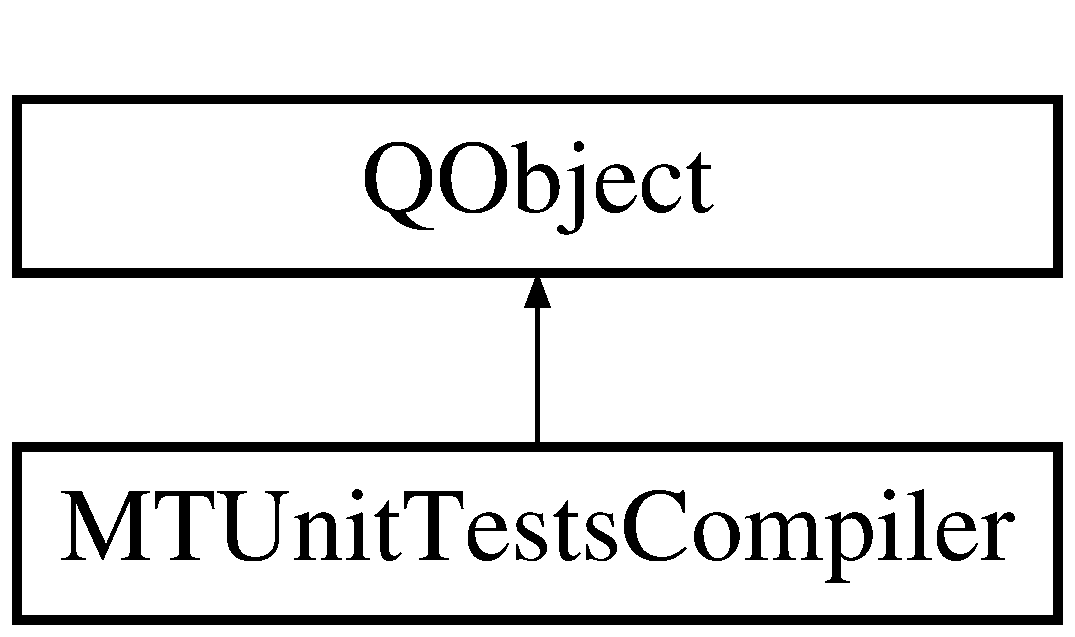
\includegraphics[height=2.000000cm]{class_m_t_unit_tests_compiler}
\end{center}
\end{figure}
\subsection*{Public Slots}
\begin{DoxyCompactItemize}
\item 
void \mbox{\hyperlink{class_m_t_unit_tests_compiler_a87e718123e996863f9eeae8e50967407}{handle\+Directory\+Changed}} (Q\+String dir)
\begin{DoxyCompactList}\small\item\em Handles inclusions or exclusions of files in the Test dir. \end{DoxyCompactList}\item 
void \mbox{\hyperlink{class_m_t_unit_tests_compiler_ad8f142f5b3dc90fbca24ba35456681be}{handle\+File\+Changed}} (Q\+String file)
\begin{DoxyCompactList}\small\item\em Handle content changes in files. \end{DoxyCompactList}\end{DoxyCompactItemize}
\subsection*{Public Member Functions}
\begin{DoxyCompactItemize}
\item 
\mbox{\hyperlink{class_m_t_unit_tests_compiler_a967536920e13cf8a653211135fd6b0e2}{M\+T\+Unit\+Tests\+Compiler}} ()
\item 
\mbox{\hyperlink{class_m_t_unit_tests_compiler_a455bbf3b47473ebb553a78421f538f23}{$\sim$\+M\+T\+Unit\+Tests\+Compiler}} ()
\item 
void \mbox{\hyperlink{class_m_t_unit_tests_compiler_afab7db9083a0cd6869b69c989898e4ee}{init\+Watcher}} (Q\+String root\+Dir)
\begin{DoxyCompactList}\small\item\em Keeps an eye on the Test directory and whenever a change is found it will automatically generates a new \mbox{\hyperlink{_m_t_unit_all_tests_8mqh}{M\+T\+Unit\+All\+Tests.\+mqh}} file. \end{DoxyCompactList}\item 
int \mbox{\hyperlink{class_m_t_unit_tests_compiler_ac87a287b33abd2f15d2af2c589afdb73}{start}} (Q\+String root\+Dir)
\begin{DoxyCompactList}\small\item\em Init the tests compilation and outputs a file called \mbox{\hyperlink{_m_t_unit_all_tests_8mqh}{M\+T\+Unit\+All\+Tests.\+mqh}}. \end{DoxyCompactList}\end{DoxyCompactItemize}


\subsection{Detailed Description}


Definition at line 32 of file mt\+Unit\+Tests\+Compiler.\+h.



\subsection{Constructor \& Destructor Documentation}
\mbox{\Hypertarget{class_m_t_unit_tests_compiler_a967536920e13cf8a653211135fd6b0e2}\label{class_m_t_unit_tests_compiler_a967536920e13cf8a653211135fd6b0e2}} 
\index{M\+T\+Unit\+Tests\+Compiler@{M\+T\+Unit\+Tests\+Compiler}!M\+T\+Unit\+Tests\+Compiler@{M\+T\+Unit\+Tests\+Compiler}}
\index{M\+T\+Unit\+Tests\+Compiler@{M\+T\+Unit\+Tests\+Compiler}!M\+T\+Unit\+Tests\+Compiler@{M\+T\+Unit\+Tests\+Compiler}}
\subsubsection{\texorpdfstring{M\+T\+Unit\+Tests\+Compiler()}{MTUnitTestsCompiler()}}
{\footnotesize\ttfamily M\+T\+Unit\+Tests\+Compiler\+::\+M\+T\+Unit\+Tests\+Compiler (\begin{DoxyParamCaption}{ }\end{DoxyParamCaption})\hspace{0.3cm}{\ttfamily [inline]}}



Definition at line 36 of file mt\+Unit\+Tests\+Compiler.\+h.

\mbox{\Hypertarget{class_m_t_unit_tests_compiler_a455bbf3b47473ebb553a78421f538f23}\label{class_m_t_unit_tests_compiler_a455bbf3b47473ebb553a78421f538f23}} 
\index{M\+T\+Unit\+Tests\+Compiler@{M\+T\+Unit\+Tests\+Compiler}!````~M\+T\+Unit\+Tests\+Compiler@{$\sim$\+M\+T\+Unit\+Tests\+Compiler}}
\index{````~M\+T\+Unit\+Tests\+Compiler@{$\sim$\+M\+T\+Unit\+Tests\+Compiler}!M\+T\+Unit\+Tests\+Compiler@{M\+T\+Unit\+Tests\+Compiler}}
\subsubsection{\texorpdfstring{$\sim$\+M\+T\+Unit\+Tests\+Compiler()}{~MTUnitTestsCompiler()}}
{\footnotesize\ttfamily M\+T\+Unit\+Tests\+Compiler\+::$\sim$\+M\+T\+Unit\+Tests\+Compiler (\begin{DoxyParamCaption}{ }\end{DoxyParamCaption})\hspace{0.3cm}{\ttfamily [inline]}}



Definition at line 37 of file mt\+Unit\+Tests\+Compiler.\+h.



\subsection{Member Function Documentation}
\mbox{\Hypertarget{class_m_t_unit_tests_compiler_a87e718123e996863f9eeae8e50967407}\label{class_m_t_unit_tests_compiler_a87e718123e996863f9eeae8e50967407}} 
\index{M\+T\+Unit\+Tests\+Compiler@{M\+T\+Unit\+Tests\+Compiler}!handle\+Directory\+Changed@{handle\+Directory\+Changed}}
\index{handle\+Directory\+Changed@{handle\+Directory\+Changed}!M\+T\+Unit\+Tests\+Compiler@{M\+T\+Unit\+Tests\+Compiler}}
\subsubsection{\texorpdfstring{handle\+Directory\+Changed}{handleDirectoryChanged}}
{\footnotesize\ttfamily void M\+T\+Unit\+Tests\+Compiler\+::handle\+Directory\+Changed (\begin{DoxyParamCaption}\item[{Q\+String}]{dir }\end{DoxyParamCaption})\hspace{0.3cm}{\ttfamily [slot]}}



Handles inclusions or exclusions of files in the Test dir. 


\begin{DoxyParams}{Parameters}
{\em dir} & \\
\hline
\end{DoxyParams}


Definition at line 44 of file mt\+Unit\+Tests\+Compiler.\+cpp.

\mbox{\Hypertarget{class_m_t_unit_tests_compiler_ad8f142f5b3dc90fbca24ba35456681be}\label{class_m_t_unit_tests_compiler_ad8f142f5b3dc90fbca24ba35456681be}} 
\index{M\+T\+Unit\+Tests\+Compiler@{M\+T\+Unit\+Tests\+Compiler}!handle\+File\+Changed@{handle\+File\+Changed}}
\index{handle\+File\+Changed@{handle\+File\+Changed}!M\+T\+Unit\+Tests\+Compiler@{M\+T\+Unit\+Tests\+Compiler}}
\subsubsection{\texorpdfstring{handle\+File\+Changed}{handleFileChanged}}
{\footnotesize\ttfamily void M\+T\+Unit\+Tests\+Compiler\+::handle\+File\+Changed (\begin{DoxyParamCaption}\item[{Q\+String}]{file }\end{DoxyParamCaption})\hspace{0.3cm}{\ttfamily [slot]}}



Handle content changes in files. 


\begin{DoxyParams}{Parameters}
{\em file} & \\
\hline
\end{DoxyParams}


Definition at line 58 of file mt\+Unit\+Tests\+Compiler.\+cpp.

\mbox{\Hypertarget{class_m_t_unit_tests_compiler_afab7db9083a0cd6869b69c989898e4ee}\label{class_m_t_unit_tests_compiler_afab7db9083a0cd6869b69c989898e4ee}} 
\index{M\+T\+Unit\+Tests\+Compiler@{M\+T\+Unit\+Tests\+Compiler}!init\+Watcher@{init\+Watcher}}
\index{init\+Watcher@{init\+Watcher}!M\+T\+Unit\+Tests\+Compiler@{M\+T\+Unit\+Tests\+Compiler}}
\subsubsection{\texorpdfstring{init\+Watcher()}{initWatcher()}}
{\footnotesize\ttfamily void M\+T\+Unit\+Tests\+Compiler\+::init\+Watcher (\begin{DoxyParamCaption}\item[{Q\+String}]{root\+Dir }\end{DoxyParamCaption})}



Keeps an eye on the Test directory and whenever a change is found it will automatically generates a new \mbox{\hyperlink{_m_t_unit_all_tests_8mqh}{M\+T\+Unit\+All\+Tests.\+mqh}} file. 


\begin{DoxyParams}{Parameters}
{\em root\+Dir} & \\
\hline
\end{DoxyParams}


Definition at line 25 of file mt\+Unit\+Tests\+Compiler.\+cpp.

\mbox{\Hypertarget{class_m_t_unit_tests_compiler_ac87a287b33abd2f15d2af2c589afdb73}\label{class_m_t_unit_tests_compiler_ac87a287b33abd2f15d2af2c589afdb73}} 
\index{M\+T\+Unit\+Tests\+Compiler@{M\+T\+Unit\+Tests\+Compiler}!start@{start}}
\index{start@{start}!M\+T\+Unit\+Tests\+Compiler@{M\+T\+Unit\+Tests\+Compiler}}
\subsubsection{\texorpdfstring{start()}{start()}}
{\footnotesize\ttfamily int M\+T\+Unit\+Tests\+Compiler\+::start (\begin{DoxyParamCaption}\item[{Q\+String}]{root\+Dir }\end{DoxyParamCaption})}



Init the tests compilation and outputs a file called \mbox{\hyperlink{_m_t_unit_all_tests_8mqh}{M\+T\+Unit\+All\+Tests.\+mqh}}. 


\begin{DoxyParams}{Parameters}
{\em root\+Dir} & \\
\hline
\end{DoxyParams}
\begin{DoxyReturn}{Returns}
The result of the procedure. (-\/1 = failure, 1 = success) 
\end{DoxyReturn}


Definition at line 73 of file mt\+Unit\+Tests\+Compiler.\+cpp.



The documentation for this class was generated from the following files\+:\begin{DoxyCompactItemize}
\item 
Source/\mbox{\hyperlink{mt_unit_tests_compiler_8h}{mt\+Unit\+Tests\+Compiler.\+h}}\item 
Source/\mbox{\hyperlink{mt_unit_tests_compiler_8cpp}{mt\+Unit\+Tests\+Compiler.\+cpp}}\end{DoxyCompactItemize}

\hypertarget{class_my_basic_test_suite}{}\section{My\+Basic\+Test\+Suite Class Reference}
\label{class_my_basic_test_suite}\index{My\+Basic\+Test\+Suite@{My\+Basic\+Test\+Suite}}


Example of Test Suite.  


\subsection*{Public Member Functions}
\begin{DoxyCompactItemize}
\item 
void \mbox{\hyperlink{class_my_basic_test_suite_a78580af3199c6d14278446ba5c67b741}{set\+Up}} ()
\begin{DoxyCompactList}\small\item\em Initializes each test case. \end{DoxyCompactList}\item 
void \mbox{\hyperlink{class_my_basic_test_suite_a83b6bce47ffac97d43b8e2d14cbd48aa}{tear\+Down}} ()
\begin{DoxyCompactList}\small\item\em Terminate each test case. \end{DoxyCompactList}\item 
void \mbox{\hyperlink{class_my_basic_test_suite_a0f9bf87994d157ca17f8cf2d8d8d31b7}{test\+\_\+bool\+\_\+assert\+True\+\_\+succeed}} ()
\item 
void \mbox{\hyperlink{class_my_basic_test_suite_ae8f4c3d56e31655ae5f887c4f73b34e6}{test\+\_\+bool\+\_\+assert\+False\+\_\+succeed}} ()
\item 
void \mbox{\hyperlink{class_my_basic_test_suite_a78e65fb1514fc53943a942d99222ef26}{test\+\_\+integers\+\_\+int\+\_\+assert\+Equals\+\_\+succeed}} ()
\item 
void \mbox{\hyperlink{class_my_basic_test_suite_af6dbaa47377dfe79f4c00a20789757ed}{test\+\_\+integers\+\_\+long\+\_\+assert\+Equals\+\_\+succeed}} ()
\item 
void \mbox{\hyperlink{class_my_basic_test_suite_ab56d6a5bc0e0ccb511798df750acb4a1}{test\+\_\+float\+\_\+assert\+Equals\+\_\+succeed}} ()
\item 
void \mbox{\hyperlink{class_my_basic_test_suite_a4e1eb8aaa161bb78d81f87ced7a34622}{test\+\_\+double\+\_\+assert\+Equals\+\_\+succeed}} ()
\item 
void \mbox{\hyperlink{class_my_basic_test_suite_ac6cfe0dda4c123f996129b55fd703865}{test\+\_\+string\+\_\+assert\+Equals\+\_\+succeed}} ()
\end{DoxyCompactItemize}


\subsection{Detailed Description}
Example of Test Suite. 

Run some basic assertions 

Definition at line 20 of file Basic\+Test\+Suite\+\_\+\+Test.\+mqh.



\subsection{Member Function Documentation}
\mbox{\Hypertarget{class_my_basic_test_suite_a78580af3199c6d14278446ba5c67b741}\label{class_my_basic_test_suite_a78580af3199c6d14278446ba5c67b741}} 
\index{My\+Basic\+Test\+Suite@{My\+Basic\+Test\+Suite}!set\+Up@{set\+Up}}
\index{set\+Up@{set\+Up}!My\+Basic\+Test\+Suite@{My\+Basic\+Test\+Suite}}
\subsubsection{\texorpdfstring{set\+Up()}{setUp()}}
{\footnotesize\ttfamily void My\+Basic\+Test\+Suite\+::set\+Up (\begin{DoxyParamCaption}{ }\end{DoxyParamCaption})\hspace{0.3cm}{\ttfamily [inline]}}



Initializes each test case. 

This is called before each test case runs 

Definition at line 27 of file Basic\+Test\+Suite\+\_\+\+Test.\+mqh.

\mbox{\Hypertarget{class_my_basic_test_suite_a83b6bce47ffac97d43b8e2d14cbd48aa}\label{class_my_basic_test_suite_a83b6bce47ffac97d43b8e2d14cbd48aa}} 
\index{My\+Basic\+Test\+Suite@{My\+Basic\+Test\+Suite}!tear\+Down@{tear\+Down}}
\index{tear\+Down@{tear\+Down}!My\+Basic\+Test\+Suite@{My\+Basic\+Test\+Suite}}
\subsubsection{\texorpdfstring{tear\+Down()}{tearDown()}}
{\footnotesize\ttfamily void My\+Basic\+Test\+Suite\+::tear\+Down (\begin{DoxyParamCaption}{ }\end{DoxyParamCaption})\hspace{0.3cm}{\ttfamily [inline]}}



Terminate each test case. 

This is called after each test case runs 

Definition at line 34 of file Basic\+Test\+Suite\+\_\+\+Test.\+mqh.

\mbox{\Hypertarget{class_my_basic_test_suite_ae8f4c3d56e31655ae5f887c4f73b34e6}\label{class_my_basic_test_suite_ae8f4c3d56e31655ae5f887c4f73b34e6}} 
\index{My\+Basic\+Test\+Suite@{My\+Basic\+Test\+Suite}!test\+\_\+bool\+\_\+assert\+False\+\_\+succeed@{test\+\_\+bool\+\_\+assert\+False\+\_\+succeed}}
\index{test\+\_\+bool\+\_\+assert\+False\+\_\+succeed@{test\+\_\+bool\+\_\+assert\+False\+\_\+succeed}!My\+Basic\+Test\+Suite@{My\+Basic\+Test\+Suite}}
\subsubsection{\texorpdfstring{test\+\_\+bool\+\_\+assert\+False\+\_\+succeed()}{test\_bool\_assertFalse\_succeed()}}
{\footnotesize\ttfamily void My\+Basic\+Test\+Suite\+::test\+\_\+bool\+\_\+assert\+False\+\_\+succeed (\begin{DoxyParamCaption}{ }\end{DoxyParamCaption})\hspace{0.3cm}{\ttfamily [inline]}}



Definition at line 45 of file Basic\+Test\+Suite\+\_\+\+Test.\+mqh.

\mbox{\Hypertarget{class_my_basic_test_suite_a0f9bf87994d157ca17f8cf2d8d8d31b7}\label{class_my_basic_test_suite_a0f9bf87994d157ca17f8cf2d8d8d31b7}} 
\index{My\+Basic\+Test\+Suite@{My\+Basic\+Test\+Suite}!test\+\_\+bool\+\_\+assert\+True\+\_\+succeed@{test\+\_\+bool\+\_\+assert\+True\+\_\+succeed}}
\index{test\+\_\+bool\+\_\+assert\+True\+\_\+succeed@{test\+\_\+bool\+\_\+assert\+True\+\_\+succeed}!My\+Basic\+Test\+Suite@{My\+Basic\+Test\+Suite}}
\subsubsection{\texorpdfstring{test\+\_\+bool\+\_\+assert\+True\+\_\+succeed()}{test\_bool\_assertTrue\_succeed()}}
{\footnotesize\ttfamily void My\+Basic\+Test\+Suite\+::test\+\_\+bool\+\_\+assert\+True\+\_\+succeed (\begin{DoxyParamCaption}{ }\end{DoxyParamCaption})\hspace{0.3cm}{\ttfamily [inline]}}



Definition at line 38 of file Basic\+Test\+Suite\+\_\+\+Test.\+mqh.

\mbox{\Hypertarget{class_my_basic_test_suite_a4e1eb8aaa161bb78d81f87ced7a34622}\label{class_my_basic_test_suite_a4e1eb8aaa161bb78d81f87ced7a34622}} 
\index{My\+Basic\+Test\+Suite@{My\+Basic\+Test\+Suite}!test\+\_\+double\+\_\+assert\+Equals\+\_\+succeed@{test\+\_\+double\+\_\+assert\+Equals\+\_\+succeed}}
\index{test\+\_\+double\+\_\+assert\+Equals\+\_\+succeed@{test\+\_\+double\+\_\+assert\+Equals\+\_\+succeed}!My\+Basic\+Test\+Suite@{My\+Basic\+Test\+Suite}}
\subsubsection{\texorpdfstring{test\+\_\+double\+\_\+assert\+Equals\+\_\+succeed()}{test\_double\_assertEquals\_succeed()}}
{\footnotesize\ttfamily void My\+Basic\+Test\+Suite\+::test\+\_\+double\+\_\+assert\+Equals\+\_\+succeed (\begin{DoxyParamCaption}{ }\end{DoxyParamCaption})\hspace{0.3cm}{\ttfamily [inline]}}



Definition at line 81 of file Basic\+Test\+Suite\+\_\+\+Test.\+mqh.

\mbox{\Hypertarget{class_my_basic_test_suite_ab56d6a5bc0e0ccb511798df750acb4a1}\label{class_my_basic_test_suite_ab56d6a5bc0e0ccb511798df750acb4a1}} 
\index{My\+Basic\+Test\+Suite@{My\+Basic\+Test\+Suite}!test\+\_\+float\+\_\+assert\+Equals\+\_\+succeed@{test\+\_\+float\+\_\+assert\+Equals\+\_\+succeed}}
\index{test\+\_\+float\+\_\+assert\+Equals\+\_\+succeed@{test\+\_\+float\+\_\+assert\+Equals\+\_\+succeed}!My\+Basic\+Test\+Suite@{My\+Basic\+Test\+Suite}}
\subsubsection{\texorpdfstring{test\+\_\+float\+\_\+assert\+Equals\+\_\+succeed()}{test\_float\_assertEquals\_succeed()}}
{\footnotesize\ttfamily void My\+Basic\+Test\+Suite\+::test\+\_\+float\+\_\+assert\+Equals\+\_\+succeed (\begin{DoxyParamCaption}{ }\end{DoxyParamCaption})\hspace{0.3cm}{\ttfamily [inline]}}



Definition at line 73 of file Basic\+Test\+Suite\+\_\+\+Test.\+mqh.

\mbox{\Hypertarget{class_my_basic_test_suite_a78e65fb1514fc53943a942d99222ef26}\label{class_my_basic_test_suite_a78e65fb1514fc53943a942d99222ef26}} 
\index{My\+Basic\+Test\+Suite@{My\+Basic\+Test\+Suite}!test\+\_\+integers\+\_\+int\+\_\+assert\+Equals\+\_\+succeed@{test\+\_\+integers\+\_\+int\+\_\+assert\+Equals\+\_\+succeed}}
\index{test\+\_\+integers\+\_\+int\+\_\+assert\+Equals\+\_\+succeed@{test\+\_\+integers\+\_\+int\+\_\+assert\+Equals\+\_\+succeed}!My\+Basic\+Test\+Suite@{My\+Basic\+Test\+Suite}}
\subsubsection{\texorpdfstring{test\+\_\+integers\+\_\+int\+\_\+assert\+Equals\+\_\+succeed()}{test\_integers\_int\_assertEquals\_succeed()}}
{\footnotesize\ttfamily void My\+Basic\+Test\+Suite\+::test\+\_\+integers\+\_\+int\+\_\+assert\+Equals\+\_\+succeed (\begin{DoxyParamCaption}{ }\end{DoxyParamCaption})\hspace{0.3cm}{\ttfamily [inline]}}



Definition at line 51 of file Basic\+Test\+Suite\+\_\+\+Test.\+mqh.

\mbox{\Hypertarget{class_my_basic_test_suite_af6dbaa47377dfe79f4c00a20789757ed}\label{class_my_basic_test_suite_af6dbaa47377dfe79f4c00a20789757ed}} 
\index{My\+Basic\+Test\+Suite@{My\+Basic\+Test\+Suite}!test\+\_\+integers\+\_\+long\+\_\+assert\+Equals\+\_\+succeed@{test\+\_\+integers\+\_\+long\+\_\+assert\+Equals\+\_\+succeed}}
\index{test\+\_\+integers\+\_\+long\+\_\+assert\+Equals\+\_\+succeed@{test\+\_\+integers\+\_\+long\+\_\+assert\+Equals\+\_\+succeed}!My\+Basic\+Test\+Suite@{My\+Basic\+Test\+Suite}}
\subsubsection{\texorpdfstring{test\+\_\+integers\+\_\+long\+\_\+assert\+Equals\+\_\+succeed()}{test\_integers\_long\_assertEquals\_succeed()}}
{\footnotesize\ttfamily void My\+Basic\+Test\+Suite\+::test\+\_\+integers\+\_\+long\+\_\+assert\+Equals\+\_\+succeed (\begin{DoxyParamCaption}{ }\end{DoxyParamCaption})\hspace{0.3cm}{\ttfamily [inline]}}



Definition at line 62 of file Basic\+Test\+Suite\+\_\+\+Test.\+mqh.

\mbox{\Hypertarget{class_my_basic_test_suite_ac6cfe0dda4c123f996129b55fd703865}\label{class_my_basic_test_suite_ac6cfe0dda4c123f996129b55fd703865}} 
\index{My\+Basic\+Test\+Suite@{My\+Basic\+Test\+Suite}!test\+\_\+string\+\_\+assert\+Equals\+\_\+succeed@{test\+\_\+string\+\_\+assert\+Equals\+\_\+succeed}}
\index{test\+\_\+string\+\_\+assert\+Equals\+\_\+succeed@{test\+\_\+string\+\_\+assert\+Equals\+\_\+succeed}!My\+Basic\+Test\+Suite@{My\+Basic\+Test\+Suite}}
\subsubsection{\texorpdfstring{test\+\_\+string\+\_\+assert\+Equals\+\_\+succeed()}{test\_string\_assertEquals\_succeed()}}
{\footnotesize\ttfamily void My\+Basic\+Test\+Suite\+::test\+\_\+string\+\_\+assert\+Equals\+\_\+succeed (\begin{DoxyParamCaption}{ }\end{DoxyParamCaption})\hspace{0.3cm}{\ttfamily [inline]}}



Definition at line 89 of file Basic\+Test\+Suite\+\_\+\+Test.\+mqh.



The documentation for this class was generated from the following file\+:\begin{DoxyCompactItemize}
\item 
Test/\mbox{\hyperlink{_basic_test_suite___test_8mqh}{Basic\+Test\+Suite\+\_\+\+Test.\+mqh}}\end{DoxyCompactItemize}

\hypertarget{class_my_class_testing_test_suite}{}\section{My\+Class\+Testing\+Test\+Suite Class Reference}
\label{class_my_class_testing_test_suite}\index{My\+Class\+Testing\+Test\+Suite@{My\+Class\+Testing\+Test\+Suite}}


Example of Test Suite.  


\subsection*{Public Member Functions}
\begin{DoxyCompactItemize}
\item 
void \mbox{\hyperlink{class_my_class_testing_test_suite_adbc1afafe2aa71c35e21f2d58d492ed8}{set\+Up}} ()
\begin{DoxyCompactList}\small\item\em Initializes each test case. \end{DoxyCompactList}\item 
void \mbox{\hyperlink{class_my_class_testing_test_suite_a57d7a3ad48dae9c768a2ec17f65503c4}{tear\+Down}} ()
\begin{DoxyCompactList}\small\item\em Terminate each test case. \end{DoxyCompactList}\item 
void \mbox{\hyperlink{class_my_class_testing_test_suite_a2f8139a2e71068665e18f99781358111}{test\+\_\+public\+Methods}} ()
\item 
void \mbox{\hyperlink{class_my_class_testing_test_suite_aadb56765b805c6dadcb2fb6d3c607e27}{test\+\_\+static\+Methods}} ()
\item 
void \mbox{\hyperlink{class_my_class_testing_test_suite_a4f3c0c96822f2d5d1a5ce80c47f156fb}{test\+\_\+private\+Methods}} ()
\end{DoxyCompactItemize}


\subsection{Detailed Description}
Example of Test Suite. 

Run some tests using direct object casting 

Definition at line 151 of file Basic\+Test\+Suite\+\_\+\+Test.\+mqh.



\subsection{Member Function Documentation}
\mbox{\Hypertarget{class_my_class_testing_test_suite_adbc1afafe2aa71c35e21f2d58d492ed8}\label{class_my_class_testing_test_suite_adbc1afafe2aa71c35e21f2d58d492ed8}} 
\index{My\+Class\+Testing\+Test\+Suite@{My\+Class\+Testing\+Test\+Suite}!set\+Up@{set\+Up}}
\index{set\+Up@{set\+Up}!My\+Class\+Testing\+Test\+Suite@{My\+Class\+Testing\+Test\+Suite}}
\subsubsection{\texorpdfstring{set\+Up()}{setUp()}}
{\footnotesize\ttfamily void My\+Class\+Testing\+Test\+Suite\+::set\+Up (\begin{DoxyParamCaption}{ }\end{DoxyParamCaption})\hspace{0.3cm}{\ttfamily [inline]}}



Initializes each test case. 

This is called before each test case runs 

Definition at line 158 of file Basic\+Test\+Suite\+\_\+\+Test.\+mqh.

\mbox{\Hypertarget{class_my_class_testing_test_suite_a57d7a3ad48dae9c768a2ec17f65503c4}\label{class_my_class_testing_test_suite_a57d7a3ad48dae9c768a2ec17f65503c4}} 
\index{My\+Class\+Testing\+Test\+Suite@{My\+Class\+Testing\+Test\+Suite}!tear\+Down@{tear\+Down}}
\index{tear\+Down@{tear\+Down}!My\+Class\+Testing\+Test\+Suite@{My\+Class\+Testing\+Test\+Suite}}
\subsubsection{\texorpdfstring{tear\+Down()}{tearDown()}}
{\footnotesize\ttfamily void My\+Class\+Testing\+Test\+Suite\+::tear\+Down (\begin{DoxyParamCaption}{ }\end{DoxyParamCaption})\hspace{0.3cm}{\ttfamily [inline]}}



Terminate each test case. 

This is called after each test case runs 

Definition at line 166 of file Basic\+Test\+Suite\+\_\+\+Test.\+mqh.

\mbox{\Hypertarget{class_my_class_testing_test_suite_a4f3c0c96822f2d5d1a5ce80c47f156fb}\label{class_my_class_testing_test_suite_a4f3c0c96822f2d5d1a5ce80c47f156fb}} 
\index{My\+Class\+Testing\+Test\+Suite@{My\+Class\+Testing\+Test\+Suite}!test\+\_\+private\+Methods@{test\+\_\+private\+Methods}}
\index{test\+\_\+private\+Methods@{test\+\_\+private\+Methods}!My\+Class\+Testing\+Test\+Suite@{My\+Class\+Testing\+Test\+Suite}}
\subsubsection{\texorpdfstring{test\+\_\+private\+Methods()}{test\_privateMethods()}}
{\footnotesize\ttfamily void My\+Class\+Testing\+Test\+Suite\+::test\+\_\+private\+Methods (\begin{DoxyParamCaption}{ }\end{DoxyParamCaption})\hspace{0.3cm}{\ttfamily [inline]}}



Definition at line 193 of file Basic\+Test\+Suite\+\_\+\+Test.\+mqh.

\mbox{\Hypertarget{class_my_class_testing_test_suite_a2f8139a2e71068665e18f99781358111}\label{class_my_class_testing_test_suite_a2f8139a2e71068665e18f99781358111}} 
\index{My\+Class\+Testing\+Test\+Suite@{My\+Class\+Testing\+Test\+Suite}!test\+\_\+public\+Methods@{test\+\_\+public\+Methods}}
\index{test\+\_\+public\+Methods@{test\+\_\+public\+Methods}!My\+Class\+Testing\+Test\+Suite@{My\+Class\+Testing\+Test\+Suite}}
\subsubsection{\texorpdfstring{test\+\_\+public\+Methods()}{test\_publicMethods()}}
{\footnotesize\ttfamily void My\+Class\+Testing\+Test\+Suite\+::test\+\_\+public\+Methods (\begin{DoxyParamCaption}{ }\end{DoxyParamCaption})\hspace{0.3cm}{\ttfamily [inline]}}



Definition at line 171 of file Basic\+Test\+Suite\+\_\+\+Test.\+mqh.

\mbox{\Hypertarget{class_my_class_testing_test_suite_aadb56765b805c6dadcb2fb6d3c607e27}\label{class_my_class_testing_test_suite_aadb56765b805c6dadcb2fb6d3c607e27}} 
\index{My\+Class\+Testing\+Test\+Suite@{My\+Class\+Testing\+Test\+Suite}!test\+\_\+static\+Methods@{test\+\_\+static\+Methods}}
\index{test\+\_\+static\+Methods@{test\+\_\+static\+Methods}!My\+Class\+Testing\+Test\+Suite@{My\+Class\+Testing\+Test\+Suite}}
\subsubsection{\texorpdfstring{test\+\_\+static\+Methods()}{test\_staticMethods()}}
{\footnotesize\ttfamily void My\+Class\+Testing\+Test\+Suite\+::test\+\_\+static\+Methods (\begin{DoxyParamCaption}{ }\end{DoxyParamCaption})\hspace{0.3cm}{\ttfamily [inline]}}



Definition at line 183 of file Basic\+Test\+Suite\+\_\+\+Test.\+mqh.



The documentation for this class was generated from the following file\+:\begin{DoxyCompactItemize}
\item 
Test/\mbox{\hyperlink{_basic_test_suite___test_8mqh}{Basic\+Test\+Suite\+\_\+\+Test.\+mqh}}\end{DoxyCompactItemize}

\hypertarget{class_my_global_scope_test_suite}{}\section{My\+Global\+Scope\+Test\+Suite Class Reference}
\label{class_my_global_scope_test_suite}\index{My\+Global\+Scope\+Test\+Suite@{My\+Global\+Scope\+Test\+Suite}}


Example of Test Suite.  


\subsection*{Public Member Functions}
\begin{DoxyCompactItemize}
\item 
void \mbox{\hyperlink{class_my_global_scope_test_suite_a21f7c76b6286f5f15cf047a5e396b17d}{set\+Up}} ()
\begin{DoxyCompactList}\small\item\em Initializes each test case. \end{DoxyCompactList}\item 
void \mbox{\hyperlink{class_my_global_scope_test_suite_aa99b3ed200fc5ff645509972190a4b29}{tear\+Down}} ()
\begin{DoxyCompactList}\small\item\em Terminate each test case. \end{DoxyCompactList}\item 
void \mbox{\hyperlink{class_my_global_scope_test_suite_a312549090f668135e117a8d6bb1160c0}{test\+\_\+\+Get\+M\+A\+\_\+shoud\+Return\+S\+MA}} ()
\item 
void \mbox{\hyperlink{class_my_global_scope_test_suite_a0b70c8c23cd8d6595cac8f6b7da3cc07}{test\+\_\+\+Get\+M\+A\+Array\+\_\+shoud\+Return\+Couple\+Of\+S\+MA}} ()
\end{DoxyCompactItemize}


\subsection{Detailed Description}
Example of Test Suite. 

Run some tests within a global scope 

Definition at line 104 of file Basic\+Test\+Suite\+\_\+\+Test.\+mqh.



\subsection{Member Function Documentation}
\mbox{\Hypertarget{class_my_global_scope_test_suite_a21f7c76b6286f5f15cf047a5e396b17d}\label{class_my_global_scope_test_suite_a21f7c76b6286f5f15cf047a5e396b17d}} 
\index{My\+Global\+Scope\+Test\+Suite@{My\+Global\+Scope\+Test\+Suite}!set\+Up@{set\+Up}}
\index{set\+Up@{set\+Up}!My\+Global\+Scope\+Test\+Suite@{My\+Global\+Scope\+Test\+Suite}}
\subsubsection{\texorpdfstring{set\+Up()}{setUp()}}
{\footnotesize\ttfamily void My\+Global\+Scope\+Test\+Suite\+::set\+Up (\begin{DoxyParamCaption}{ }\end{DoxyParamCaption})\hspace{0.3cm}{\ttfamily [inline]}}



Initializes each test case. 

This is called before each test case runs 

Definition at line 111 of file Basic\+Test\+Suite\+\_\+\+Test.\+mqh.

\mbox{\Hypertarget{class_my_global_scope_test_suite_aa99b3ed200fc5ff645509972190a4b29}\label{class_my_global_scope_test_suite_aa99b3ed200fc5ff645509972190a4b29}} 
\index{My\+Global\+Scope\+Test\+Suite@{My\+Global\+Scope\+Test\+Suite}!tear\+Down@{tear\+Down}}
\index{tear\+Down@{tear\+Down}!My\+Global\+Scope\+Test\+Suite@{My\+Global\+Scope\+Test\+Suite}}
\subsubsection{\texorpdfstring{tear\+Down()}{tearDown()}}
{\footnotesize\ttfamily void My\+Global\+Scope\+Test\+Suite\+::tear\+Down (\begin{DoxyParamCaption}{ }\end{DoxyParamCaption})\hspace{0.3cm}{\ttfamily [inline]}}



Terminate each test case. 

This is called after each test case runs 

Definition at line 118 of file Basic\+Test\+Suite\+\_\+\+Test.\+mqh.

\mbox{\Hypertarget{class_my_global_scope_test_suite_a312549090f668135e117a8d6bb1160c0}\label{class_my_global_scope_test_suite_a312549090f668135e117a8d6bb1160c0}} 
\index{My\+Global\+Scope\+Test\+Suite@{My\+Global\+Scope\+Test\+Suite}!test\+\_\+\+Get\+M\+A\+\_\+shoud\+Return\+S\+MA@{test\+\_\+\+Get\+M\+A\+\_\+shoud\+Return\+S\+MA}}
\index{test\+\_\+\+Get\+M\+A\+\_\+shoud\+Return\+S\+MA@{test\+\_\+\+Get\+M\+A\+\_\+shoud\+Return\+S\+MA}!My\+Global\+Scope\+Test\+Suite@{My\+Global\+Scope\+Test\+Suite}}
\subsubsection{\texorpdfstring{test\+\_\+\+Get\+M\+A\+\_\+shoud\+Return\+S\+M\+A()}{test\_GetMA\_shoudReturnSMA()}}
{\footnotesize\ttfamily void My\+Global\+Scope\+Test\+Suite\+::test\+\_\+\+Get\+M\+A\+\_\+shoud\+Return\+S\+MA (\begin{DoxyParamCaption}{ }\end{DoxyParamCaption})\hspace{0.3cm}{\ttfamily [inline]}}



Definition at line 122 of file Basic\+Test\+Suite\+\_\+\+Test.\+mqh.

\mbox{\Hypertarget{class_my_global_scope_test_suite_a0b70c8c23cd8d6595cac8f6b7da3cc07}\label{class_my_global_scope_test_suite_a0b70c8c23cd8d6595cac8f6b7da3cc07}} 
\index{My\+Global\+Scope\+Test\+Suite@{My\+Global\+Scope\+Test\+Suite}!test\+\_\+\+Get\+M\+A\+Array\+\_\+shoud\+Return\+Couple\+Of\+S\+MA@{test\+\_\+\+Get\+M\+A\+Array\+\_\+shoud\+Return\+Couple\+Of\+S\+MA}}
\index{test\+\_\+\+Get\+M\+A\+Array\+\_\+shoud\+Return\+Couple\+Of\+S\+MA@{test\+\_\+\+Get\+M\+A\+Array\+\_\+shoud\+Return\+Couple\+Of\+S\+MA}!My\+Global\+Scope\+Test\+Suite@{My\+Global\+Scope\+Test\+Suite}}
\subsubsection{\texorpdfstring{test\+\_\+\+Get\+M\+A\+Array\+\_\+shoud\+Return\+Couple\+Of\+S\+M\+A()}{test\_GetMAArray\_shoudReturnCoupleOfSMA()}}
{\footnotesize\ttfamily void My\+Global\+Scope\+Test\+Suite\+::test\+\_\+\+Get\+M\+A\+Array\+\_\+shoud\+Return\+Couple\+Of\+S\+MA (\begin{DoxyParamCaption}{ }\end{DoxyParamCaption})\hspace{0.3cm}{\ttfamily [inline]}}



Definition at line 131 of file Basic\+Test\+Suite\+\_\+\+Test.\+mqh.



The documentation for this class was generated from the following file\+:\begin{DoxyCompactItemize}
\item 
Test/\mbox{\hyperlink{_basic_test_suite___test_8mqh}{Basic\+Test\+Suite\+\_\+\+Test.\+mqh}}\end{DoxyCompactItemize}

\hypertarget{class_my_inherited_test_suite}{}\section{My\+Inherited\+Test\+Suite Class Reference}
\label{class_my_inherited_test_suite}\index{My\+Inherited\+Test\+Suite@{My\+Inherited\+Test\+Suite}}


Example of Test Suite.  


Inheritance diagram for My\+Inherited\+Test\+Suite\+:\begin{figure}[H]
\begin{center}
\leavevmode
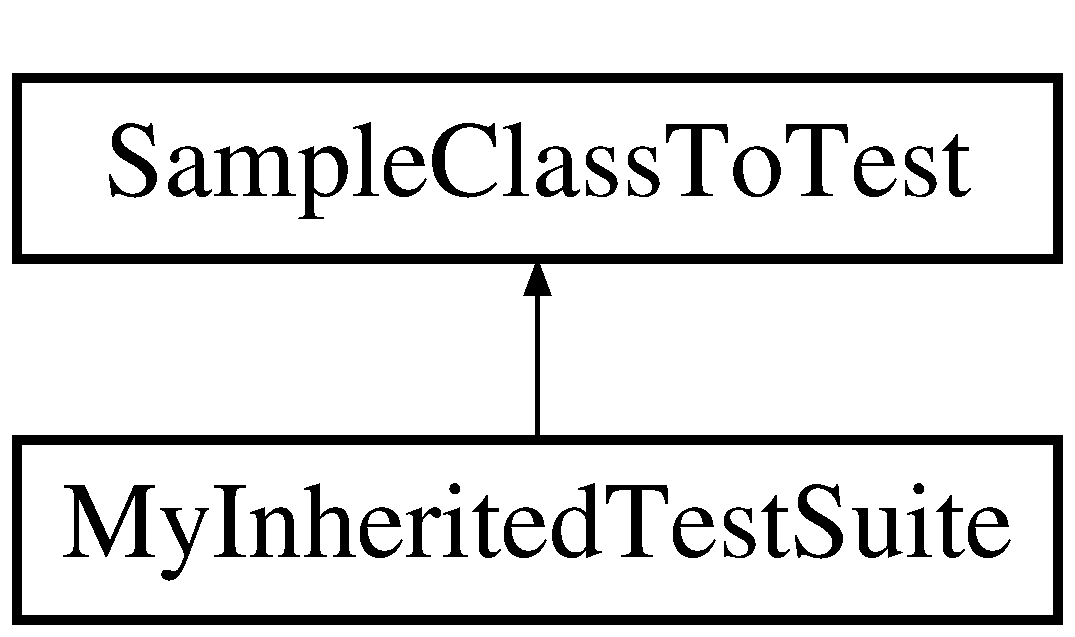
\includegraphics[height=2.000000cm]{class_my_inherited_test_suite}
\end{center}
\end{figure}
\subsection*{Public Member Functions}
\begin{DoxyCompactItemize}
\item 
void \mbox{\hyperlink{class_my_inherited_test_suite_a3aa9d1d4ab762d55cfee1d2f6298c3f9}{set\+Up}} ()
\begin{DoxyCompactList}\small\item\em Initializes each test case. \end{DoxyCompactList}\item 
void \mbox{\hyperlink{class_my_inherited_test_suite_abbd94d1b4868f8252b001ce743eeb691}{tear\+Down}} ()
\begin{DoxyCompactList}\small\item\em Terminate each test case. \end{DoxyCompactList}\item 
void \mbox{\hyperlink{class_my_inherited_test_suite_a1a6a926a8fb9d03618008b6d882a1cfe}{test\+\_\+public\+Inherited\+Methods}} ()
\item 
void \mbox{\hyperlink{class_my_inherited_test_suite_a7fef4b3ee5331b5454ce3b6b66813e6d}{test\+\_\+protected\+Inherited\+Methods}} ()
\item 
void \mbox{\hyperlink{class_my_inherited_test_suite_a17797338b2152e4c8d5354f2efd30692}{test\+\_\+private\+Inherited\+Methods}} ()
\end{DoxyCompactItemize}


\subsection{Detailed Description}
Example of Test Suite. 

Run some tests inherited from a parent class 

Definition at line 207 of file Basic\+Test\+Suite\+\_\+\+Test.\+mqh.



\subsection{Member Function Documentation}
\mbox{\Hypertarget{class_my_inherited_test_suite_a3aa9d1d4ab762d55cfee1d2f6298c3f9}\label{class_my_inherited_test_suite_a3aa9d1d4ab762d55cfee1d2f6298c3f9}} 
\index{My\+Inherited\+Test\+Suite@{My\+Inherited\+Test\+Suite}!set\+Up@{set\+Up}}
\index{set\+Up@{set\+Up}!My\+Inherited\+Test\+Suite@{My\+Inherited\+Test\+Suite}}
\subsubsection{\texorpdfstring{set\+Up()}{setUp()}}
{\footnotesize\ttfamily void My\+Inherited\+Test\+Suite\+::set\+Up (\begin{DoxyParamCaption}{ }\end{DoxyParamCaption})\hspace{0.3cm}{\ttfamily [inline]}}



Initializes each test case. 

This is called before each test case runs 

Definition at line 214 of file Basic\+Test\+Suite\+\_\+\+Test.\+mqh.

\mbox{\Hypertarget{class_my_inherited_test_suite_abbd94d1b4868f8252b001ce743eeb691}\label{class_my_inherited_test_suite_abbd94d1b4868f8252b001ce743eeb691}} 
\index{My\+Inherited\+Test\+Suite@{My\+Inherited\+Test\+Suite}!tear\+Down@{tear\+Down}}
\index{tear\+Down@{tear\+Down}!My\+Inherited\+Test\+Suite@{My\+Inherited\+Test\+Suite}}
\subsubsection{\texorpdfstring{tear\+Down()}{tearDown()}}
{\footnotesize\ttfamily void My\+Inherited\+Test\+Suite\+::tear\+Down (\begin{DoxyParamCaption}{ }\end{DoxyParamCaption})\hspace{0.3cm}{\ttfamily [inline]}}



Terminate each test case. 

This is called after each test case runs 

Definition at line 221 of file Basic\+Test\+Suite\+\_\+\+Test.\+mqh.

\mbox{\Hypertarget{class_my_inherited_test_suite_a17797338b2152e4c8d5354f2efd30692}\label{class_my_inherited_test_suite_a17797338b2152e4c8d5354f2efd30692}} 
\index{My\+Inherited\+Test\+Suite@{My\+Inherited\+Test\+Suite}!test\+\_\+private\+Inherited\+Methods@{test\+\_\+private\+Inherited\+Methods}}
\index{test\+\_\+private\+Inherited\+Methods@{test\+\_\+private\+Inherited\+Methods}!My\+Inherited\+Test\+Suite@{My\+Inherited\+Test\+Suite}}
\subsubsection{\texorpdfstring{test\+\_\+private\+Inherited\+Methods()}{test\_privateInheritedMethods()}}
{\footnotesize\ttfamily void My\+Inherited\+Test\+Suite\+::test\+\_\+private\+Inherited\+Methods (\begin{DoxyParamCaption}{ }\end{DoxyParamCaption})\hspace{0.3cm}{\ttfamily [inline]}}



Definition at line 235 of file Basic\+Test\+Suite\+\_\+\+Test.\+mqh.

\mbox{\Hypertarget{class_my_inherited_test_suite_a7fef4b3ee5331b5454ce3b6b66813e6d}\label{class_my_inherited_test_suite_a7fef4b3ee5331b5454ce3b6b66813e6d}} 
\index{My\+Inherited\+Test\+Suite@{My\+Inherited\+Test\+Suite}!test\+\_\+protected\+Inherited\+Methods@{test\+\_\+protected\+Inherited\+Methods}}
\index{test\+\_\+protected\+Inherited\+Methods@{test\+\_\+protected\+Inherited\+Methods}!My\+Inherited\+Test\+Suite@{My\+Inherited\+Test\+Suite}}
\subsubsection{\texorpdfstring{test\+\_\+protected\+Inherited\+Methods()}{test\_protectedInheritedMethods()}}
{\footnotesize\ttfamily void My\+Inherited\+Test\+Suite\+::test\+\_\+protected\+Inherited\+Methods (\begin{DoxyParamCaption}{ }\end{DoxyParamCaption})\hspace{0.3cm}{\ttfamily [inline]}}



Definition at line 230 of file Basic\+Test\+Suite\+\_\+\+Test.\+mqh.

\mbox{\Hypertarget{class_my_inherited_test_suite_a1a6a926a8fb9d03618008b6d882a1cfe}\label{class_my_inherited_test_suite_a1a6a926a8fb9d03618008b6d882a1cfe}} 
\index{My\+Inherited\+Test\+Suite@{My\+Inherited\+Test\+Suite}!test\+\_\+public\+Inherited\+Methods@{test\+\_\+public\+Inherited\+Methods}}
\index{test\+\_\+public\+Inherited\+Methods@{test\+\_\+public\+Inherited\+Methods}!My\+Inherited\+Test\+Suite@{My\+Inherited\+Test\+Suite}}
\subsubsection{\texorpdfstring{test\+\_\+public\+Inherited\+Methods()}{test\_publicInheritedMethods()}}
{\footnotesize\ttfamily void My\+Inherited\+Test\+Suite\+::test\+\_\+public\+Inherited\+Methods (\begin{DoxyParamCaption}{ }\end{DoxyParamCaption})\hspace{0.3cm}{\ttfamily [inline]}}



Definition at line 225 of file Basic\+Test\+Suite\+\_\+\+Test.\+mqh.



The documentation for this class was generated from the following file\+:\begin{DoxyCompactItemize}
\item 
Test/\mbox{\hyperlink{_basic_test_suite___test_8mqh}{Basic\+Test\+Suite\+\_\+\+Test.\+mqh}}\end{DoxyCompactItemize}

\chapter{File Documentation}
\hypertarget{_m_t_unit_all_tests_8mqh}{}\section{Include/\+M\+T\+Unit\+All\+Tests.mqh File Reference}
\label{_m_t_unit_all_tests_8mqh}\index{Include/\+M\+T\+Unit\+All\+Tests.\+mqh@{Include/\+M\+T\+Unit\+All\+Tests.\+mqh}}


This file is auto generated. It contains all tests that the unit test will run.  


{\ttfamily \#include \char`\"{}../\+Include/\+M\+T\+Unit.\+mqh\char`\"{}}\newline
{\ttfamily \#include \char`\"{}../\+Include/\+M\+T\+Unit\+Cfg.\+mqh\char`\"{}}\newline
{\ttfamily \#include \char`\"{}../\+Test/\+Basic\+Test\+Suite\+\_\+\+Test.\+mqh\char`\"{}}\newline
\subsection*{Classes}
\begin{DoxyCompactItemize}
\item 
class \mbox{\hyperlink{class_m_t_unit_all_tests}{M\+T\+Unit\+All\+Tests}}
\end{DoxyCompactItemize}


\subsection{Detailed Description}
This file is auto generated. It contains all tests that the unit test will run. 

\begin{DoxyAuthor}{Author}
Rodrigo Haller 
\end{DoxyAuthor}
\begin{DoxyDate}{Date}
24/02/2018 
\end{DoxyDate}

\hypertarget{_r_e_a_d_m_e_8md}{}\section{R\+E\+A\+D\+M\+E.\+md File Reference}
\label{_r_e_a_d_m_e_8md}\index{R\+E\+A\+D\+M\+E.\+md@{R\+E\+A\+D\+M\+E.\+md}}

\hypertarget{main_8cpp}{}\section{Source/main.cpp File Reference}
\label{main_8cpp}\index{Source/main.\+cpp@{Source/main.\+cpp}}


This app was made to automate Unit Testing in M\+Q\+L5.  


{\ttfamily \#include $<$Q\+Core\+Application$>$}\newline
{\ttfamily \#include $<$Q\+Thread$>$}\newline
{\ttfamily \#include $<$Q\+Debug$>$}\newline
{\ttfamily \#include \char`\"{}mt\+Unit\+E\+A\+Linker.\+h\char`\"{}}\newline
{\ttfamily \#include \char`\"{}mt\+Unit\+Logger.\+h\char`\"{}}\newline
{\ttfamily \#include \char`\"{}mt\+Unit\+Tests\+Compiler.\+h\char`\"{}}\newline
\subsection*{Functions}
\begin{DoxyCompactItemize}
\item 
int \mbox{\hyperlink{main_8cpp_a0ddf1224851353fc92bfbff6f499fa97}{main}} (int argc, char $\ast$argv\mbox{[}$\,$\mbox{]})
\begin{DoxyCompactList}\small\item\em Main method that will parse the received arguments and call the correct handler. \end{DoxyCompactList}\end{DoxyCompactItemize}


\subsection{Detailed Description}
This app was made to automate Unit Testing in M\+Q\+L5. 

\begin{DoxyAuthor}{Author}
Rodrigo Haller 
\end{DoxyAuthor}
\begin{DoxyDate}{Date}
24/02/2018
\end{DoxyDate}
It contains 3 tools that make the wholw process totally automatic. Each tool is better explained in the Readme and in their respective classes. 

\subsection{Function Documentation}
\mbox{\Hypertarget{main_8cpp_a0ddf1224851353fc92bfbff6f499fa97}\label{main_8cpp_a0ddf1224851353fc92bfbff6f499fa97}} 
\index{main.\+cpp@{main.\+cpp}!main@{main}}
\index{main@{main}!main.\+cpp@{main.\+cpp}}
\subsubsection{\texorpdfstring{main()}{main()}}
{\footnotesize\ttfamily int main (\begin{DoxyParamCaption}\item[{int}]{argc,  }\item[{char $\ast$}]{argv\mbox{[}$\,$\mbox{]} }\end{DoxyParamCaption})}



Main method that will parse the received arguments and call the correct handler. 


\begin{DoxyParams}{Parameters}
{\em argc} & \\
\hline
{\em argv} & \\
\hline
\end{DoxyParams}
\begin{DoxyReturn}{Returns}
(-\/1 = failure, 1 = success) 
\end{DoxyReturn}


Definition at line 27 of file main.\+cpp.


\hypertarget{mt_unit_e_a_linker_8cpp}{}\section{Source/mt\+Unit\+E\+A\+Linker.cpp File Reference}
\label{mt_unit_e_a_linker_8cpp}\index{Source/mt\+Unit\+E\+A\+Linker.\+cpp@{Source/mt\+Unit\+E\+A\+Linker.\+cpp}}


Update the config filed required by the Meta\+Terminal when running an Expert Advisor.  


{\ttfamily \#include \char`\"{}mt\+Unit\+E\+A\+Linker.\+h\char`\"{}}\newline


\subsection{Detailed Description}
Update the config filed required by the Meta\+Terminal when running an Expert Advisor. 

\begin{DoxyAuthor}{Author}
Rodrigo Haller 
\end{DoxyAuthor}
\begin{DoxyDate}{Date}
24/02/2018
\end{DoxyDate}
This class is used to update the config filed required by the Meta\+Terminal when running an Expert Advisor. It looks for the EA Parameter and updates it with the name of the generated .ex5 file. \begin{DoxyNote}{Note}
In order to use this class, the argument received by mt\+Unit\+Helper.\+exe must be\+: mt\+Unit\+E\+A\+Linker Path\+Of\+The\+E\+A.\+mq5\+File 
\end{DoxyNote}

\hypertarget{mt_unit_e_a_linker_8h}{}\section{Source/mt\+Unit\+E\+A\+Linker.h File Reference}
\label{mt_unit_e_a_linker_8h}\index{Source/mt\+Unit\+E\+A\+Linker.\+h@{Source/mt\+Unit\+E\+A\+Linker.\+h}}


Update the config filed required by the Meta\+Terminal when running an Expert Advisor.  


{\ttfamily \#include $<$Q\+Dir$>$}\newline
{\ttfamily \#include $<$Q\+File$>$}\newline
{\ttfamily \#include $<$Q\+File\+Info$>$}\newline
{\ttfamily \#include $<$Q\+Text\+Stream$>$}\newline
{\ttfamily \#include $<$Q\+Debug$>$}\newline
\subsection*{Classes}
\begin{DoxyCompactItemize}
\item 
class \mbox{\hyperlink{class_m_t_unit_e_a_linker}{M\+T\+Unit\+E\+A\+Linker}}
\end{DoxyCompactItemize}


\subsection{Detailed Description}
Update the config filed required by the Meta\+Terminal when running an Expert Advisor. 

\begin{DoxyAuthor}{Author}
Rodrigo Haller 
\end{DoxyAuthor}
\begin{DoxyDate}{Date}
24/02/2018
\end{DoxyDate}
This class is used to update the config filed required by the Meta\+Terminal when running an Expert Advisor. It looks for the EA Parameter and updates it with the name of the generated .ex5 file. \begin{DoxyNote}{Note}
In order to use this class, the argument received by mt\+Unit\+Helper.\+exe must be\+: mt\+Unit\+E\+A\+Linker Path\+Of\+The\+E\+A.\+mq5\+File 
\end{DoxyNote}

\hypertarget{mt_unit_logger_8cpp}{}\section{Source/mt\+Unit\+Logger.cpp File Reference}
\label{mt_unit_logger_8cpp}\index{Source/mt\+Unit\+Logger.\+cpp@{Source/mt\+Unit\+Logger.\+cpp}}


Hijacks the Log\+File and add colors to the output.  


{\ttfamily \#include \char`\"{}mt\+Unit\+Logger.\+h\char`\"{}}\newline


\subsection{Detailed Description}
Hijacks the Log\+File and add colors to the output. 

\begin{DoxyAuthor}{Author}
Rodrigo Haller 
\end{DoxyAuthor}
\begin{DoxyDate}{Date}
24/02/2018
\end{DoxyDate}
This class looks for the output log file generated by Meta\+Editor, hijacks this file to the Runners folder and adds some color to the output to make it more visual effective. \begin{DoxyNote}{Note}
In order to use this class, the argument received by mt\+Unit\+Helper.\+exe must be\+: mt\+Unit\+Logger 
\end{DoxyNote}
\begin{DoxyWarning}{Warning}
The colored output does not work directly from Meta\+Editor, so if you want to use it, I suggest you to follow the instructions for using this tool in Sublime Text 3. 
\end{DoxyWarning}

\hypertarget{mt_unitlogger_8h}{}\section{Source/mt\+Unitlogger.h File Reference}
\label{mt_unitlogger_8h}\index{Source/mt\+Unitlogger.\+h@{Source/mt\+Unitlogger.\+h}}


Hijacks the Log\+File and add colors to the output.  


{\ttfamily \#include $<$Q\+Dir$>$}\newline
{\ttfamily \#include $<$Q\+File$>$}\newline
{\ttfamily \#include $<$Q\+File\+Info$>$}\newline
{\ttfamily \#include $<$Q\+Date\+Time$>$}\newline
{\ttfamily \#include $<$Q\+String$>$}\newline
{\ttfamily \#include $<$Q\+Debug$>$}\newline
\subsection*{Classes}
\begin{DoxyCompactItemize}
\item 
class \mbox{\hyperlink{class_m_t_unit_logger}{M\+T\+Unit\+Logger}}
\end{DoxyCompactItemize}


\subsection{Detailed Description}
Hijacks the Log\+File and add colors to the output. 

\begin{DoxyAuthor}{Author}
Rodrigo Haller 
\end{DoxyAuthor}
\begin{DoxyDate}{Date}
24/02/2018
\end{DoxyDate}
This class looks for the output log file generated by Meta\+Editor, hijacks this file to the Runners folder and adds some color to the output to make it more visual effective. \begin{DoxyNote}{Note}
In order to use this class, the argument received by mt\+Unit\+Helper.\+exe must be\+: mt\+Unit\+Logger 
\end{DoxyNote}
\begin{DoxyWarning}{Warning}
The colored output does not work directly from Meta\+Editor, so if you want to use it, I suggest you to follow the instructions for using this tool in Sublime Text 3. 
\end{DoxyWarning}

\hypertarget{mt_unit_tests_compiler_8cpp}{}\section{Source/mt\+Unit\+Tests\+Compiler.cpp File Reference}
\label{mt_unit_tests_compiler_8cpp}\index{Source/mt\+Unit\+Tests\+Compiler.\+cpp@{Source/mt\+Unit\+Tests\+Compiler.\+cpp}}


Scan all Test Files and generates the \mbox{\hyperlink{_m_t_unit_all_tests_8mqh}{M\+T\+Unit\+All\+Tests.\+mqh}} file.  


{\ttfamily \#include \char`\"{}mt\+Unit\+Tests\+Compiler.\+h\char`\"{}}\newline


\subsection{Detailed Description}
Scan all Test Files and generates the \mbox{\hyperlink{_m_t_unit_all_tests_8mqh}{M\+T\+Unit\+All\+Tests.\+mqh}} file. 

\begin{DoxyAuthor}{Author}
Rodrigo Haller 
\end{DoxyAuthor}
\begin{DoxyDate}{Date}
24/02/2018
\end{DoxyDate}
This class scan the Test folder looking for all included Test Suites and Test Cases. Then it writes a file called \mbox{\hyperlink{_m_t_unit_all_tests_8mqh}{M\+T\+Unit\+All\+Tests.\+mqh}} containing all basic declarations you would have had to write manually. There is also a Watcher that monitors the Test folder and trigger the start method whenever a change is made to that directory. \begin{DoxyNote}{Note}
In order to use this class, the argument received by mt\+Unit\+Helper.\+exe must be\+: mt\+Unit\+Tests\+Compiler 

This class can also be executed in Watcher mode, to enter this mode, do not pass any argument to my\+Unit\+Helper.\+exe 
\end{DoxyNote}
\begin{DoxyWarning}{Warning}
In this case, the app will keep running until you close it. 
\end{DoxyWarning}

\hypertarget{mt_unit_tests_compiler_8h}{}\section{Source/mt\+Unit\+Tests\+Compiler.h File Reference}
\label{mt_unit_tests_compiler_8h}\index{Source/mt\+Unit\+Tests\+Compiler.\+h@{Source/mt\+Unit\+Tests\+Compiler.\+h}}


Scan all Test Files and generates the \mbox{\hyperlink{_m_t_unit_all_tests_8mqh}{M\+T\+Unit\+All\+Tests.\+mqh}} file.  


{\ttfamily \#include $<$Q\+Object$>$}\newline
{\ttfamily \#include $<$Q\+Map$>$}\newline
{\ttfamily \#include $<$Q\+Dir$>$}\newline
{\ttfamily \#include $<$Q\+File$>$}\newline
{\ttfamily \#include $<$Q\+File\+Info$>$}\newline
{\ttfamily \#include $<$Q\+Date\+Time$>$}\newline
{\ttfamily \#include $<$Q\+String\+List$>$}\newline
{\ttfamily \#include $<$Q\+Text\+Stream$>$}\newline
{\ttfamily \#include $<$Q\+File\+System\+Watcher$>$}\newline
{\ttfamily \#include $<$Q\+Debug$>$}\newline
\subsection*{Classes}
\begin{DoxyCompactItemize}
\item 
class \mbox{\hyperlink{class_m_t_unit_tests_compiler}{M\+T\+Unit\+Tests\+Compiler}}
\end{DoxyCompactItemize}


\subsection{Detailed Description}
Scan all Test Files and generates the \mbox{\hyperlink{_m_t_unit_all_tests_8mqh}{M\+T\+Unit\+All\+Tests.\+mqh}} file. 

\begin{DoxyAuthor}{Author}
Rodrigo Haller 
\end{DoxyAuthor}
\begin{DoxyDate}{Date}
24/02/2018
\end{DoxyDate}
This class scan the Test folder looking for all included Test Suites and Test Cases. Then it writes a file called \mbox{\hyperlink{_m_t_unit_all_tests_8mqh}{M\+T\+Unit\+All\+Tests.\+mqh}} containing all basic declarations you would have had to write manually. There is also a Watcher that monitors the Test folder and trigger the start method whenever a change is made to that directory. \begin{DoxyNote}{Note}
In order to use this class, the argument received by mt\+Unit\+Helper.\+exe must be\+: mt\+Unit\+Tests\+Compiler 

This class can also be executed in Watcher mode, to enter this mode, do not pass any argument to my\+Unit\+Helper.\+exe 
\end{DoxyNote}
\begin{DoxyWarning}{Warning}
In this case, the app will keep running until you close it. 
\end{DoxyWarning}

\hypertarget{_basic_test_suite___test_8mqh}{}\section{Test/\+Basic\+Test\+Suite\+\_\+\+Test.mqh File Reference}
\label{_basic_test_suite___test_8mqh}\index{Test/\+Basic\+Test\+Suite\+\_\+\+Test.\+mqh@{Test/\+Basic\+Test\+Suite\+\_\+\+Test.\+mqh}}


File containing the implementation of all Unit Test methods.  


{\ttfamily \#include \char`\"{}../\+Include/\+M\+T\+Unit.\+mqh\char`\"{}}\newline
{\ttfamily \#include \char`\"{}../\+Include/\+Sample\+Class\+To\+Test.\+mqh\char`\"{}}\newline
\subsection*{Classes}
\begin{DoxyCompactItemize}
\item 
class \mbox{\hyperlink{class_my_basic_test_suite}{My\+Basic\+Test\+Suite}}
\begin{DoxyCompactList}\small\item\em Example of Test Suite. \end{DoxyCompactList}\item 
class \mbox{\hyperlink{class_my_global_scope_test_suite}{My\+Global\+Scope\+Test\+Suite}}
\begin{DoxyCompactList}\small\item\em Example of Test Suite. \end{DoxyCompactList}\item 
class \mbox{\hyperlink{class_my_class_testing_test_suite}{My\+Class\+Testing\+Test\+Suite}}
\begin{DoxyCompactList}\small\item\em Example of Test Suite. \end{DoxyCompactList}\item 
class \mbox{\hyperlink{class_my_inherited_test_suite}{My\+Inherited\+Test\+Suite}}
\begin{DoxyCompactList}\small\item\em Example of Test Suite. \end{DoxyCompactList}\end{DoxyCompactItemize}


\subsection{Detailed Description}
File containing the implementation of all Unit Test methods. 

\begin{DoxyAuthor}{Author}
Rodrigo Haller 
\end{DoxyAuthor}
\begin{DoxyDate}{Date}
09/02/2018 
\end{DoxyDate}

%--- End generated contents ---

% Index
\backmatter
\newpage
\phantomsection
\clearemptydoublepage
\addcontentsline{toc}{chapter}{Index}
\printindex

\end{document}
